%% Slides for ".NET Programming" by Chunyu Wang <chunyu@hit.edu.cn> %%

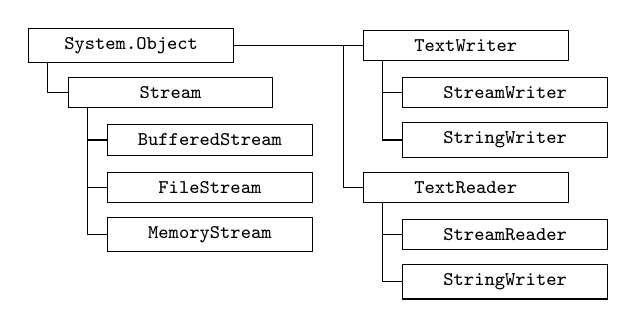
\begin{tikzpicture}
\tikzstyle{every node}=[anchor=west,draw,minimum width=2.6cm,fill=white,font=\ttfamily\scriptsize]
\node at (0,5) (a) {System.Object};
\node at (.5,4.4) (b) {Stream};
\node at (1,3.8) (b1) {BufferedStream};
\node at (1,3.2) (b2) {FileStream};
\node at (1,2.6) (b3) {MemoryStream};

\draw (a.south west) +(right:.25cm) |- (b);

\foreach \a in {b1,b2,b3}
\draw (b.south west) +(right:.25cm) |- (\a);

\node at (4.25,5)   (c) {TextWriter};
\node at (4.75,4.4)  (c1) {StreamWriter};
\node at (4.75,3.8)  (c2) {StringWriter};
\node at (4.25,3.2) (d) {TextReader};
\node at (4.75,2.6)  (d1) {StreamReader};
\node at (4.75,2)    (d2) {StringWriter};

\draw (c.south west) +(right:.25cm) |- (c1);
\draw (c.south west) +(right:.25cm) |- (c2);
\draw (d.south west) +(right:.25cm) |- (d1);
\draw (d.south west) +(right:.25cm) |- (d2);

\draw (a.east) -- (c.west);
\draw (c.west) +(left:.25cm) |- (d);

\end{tikzpicture}
